% Lesson: AlfDROID, an old OnePlus 6 turned into an always-on server on the tailnet.
% Compile with:  latexmk  (settings in .latexmkrc)

\documentclass[11pt,a4paper]{article}

\usepackage{fontspec}
\usepackage[margin=2.2cm]{geometry}
\usepackage{xcolor}
\usepackage[most]{tcolorbox}
\usepackage{listings}
\usepackage{twemojis}
\usepackage{alfdoc}
\usepackage[inline]{enumitem}
\usepackage{booktabs}
\usepackage{tikz}
\usetikzlibrary{positioning}
\usepackage[colorlinks=true,linkcolor=blue,urlcolor=blue]{hyperref}

% Recorded output is terminal output: Menlo keeps the look honest and carries the
% glyphs Latin Modern Mono lacks (✓ U+2713, the block art U+2580/84/88, ← and …).
\newfontface\termfont{Menlo}[Scale=MatchLowercase]
% ✓ must arrive through literate: listings defers unknown Unicode characters, which
% emitted every tick at the end of the previous line instead of its own.
\newcommand{\tick}{\hbox{\termfont ✓\char32}}
\lstdefinestyle{out}{
  basicstyle=\termfont\scriptsize\color{black!80}, columns=fullflexible, keepspaces=true,
  breaklines=true, breakatwhitespace=false, showstringspaces=false,
  moredelim=[is][\color{red!80!black}]{|!}{!|},
  moredelim=[is][\color{black!35}]{|~}{~|},
  literate={×}{{$\times$}}1 {→}{{$\rightarrow$}}1, escapechar=^
}

\setlength{\parindent}{0pt}
\setlength{\parskip}{0.6em}
\setlength{\emergencystretch}{3em}

\title{\emo{mobile phone}\ \name{AlfDROID}\\[0.3em]
  \large A OnePlus 6 from the drawer as an always-on server on the tailnet}
\author{Lesson for Alf, written by Claude}
\date{Tue 10 Nov 2026}

\begin{document}
\maketitle

\section*{The phone}

\name{AlfDROID} is the OnePlus 6 I bought on 31 Jul 2018, in Silk White, with 8 GB of RAM and 128 GB of storage~\cite{gsm}. Its model number is \name{A6003}, the version for Europe and North America.\here[model moved here] It sits plugged in behind the router with the screen off and joins the tailnet, so every machine of mine reaches it by name while the router keeps all its ports closed. During a power cut it keeps running on its own battery, so its programs carry on where they were. The router goes down with the power, though, so for that time the phone is unreachable and its services are offline; they answer again as soon as the router is back.

\here[SIM] A SIM card would keep the phone reachable through a power cut, because \name{Tailscale} also works over mobile data. The phone takes only physical nano-SIM cards, two of them: it has no eSIM chip, since it lists no \texttt{android.hardware.telephony.euicc} feature, so the iPhone's eSIM cannot move to it.\here[no eSIM] A plan reaches a second phone through a second SIM from the carrier, usually sold as a data-only line on the same account.

\begin{center}\small
\begin{tabular}{@{}ll@{}}
\toprule
Chip & \name{Snapdragon 845}: 8 cores, 4 at 2.8 GHz and 4 at 1.7 GHz, 64-bit Arm \\
Memory, storage & 8 GB LPDDR4X, 128 GB UFS 2.1 \\
Network & Wi-Fi 5 (802.11ac, 2$\times$2), Bluetooth 5.0 \\
Power & 3300 mAh battery; Dash Charge at 5 V, 4 A \\
Port & USB-C 2.0, which can host a USB drive, an Ethernet adapter, or my own hardware \\
Software & last official release \name{OxygenOS} 11.1.2.2 (Android 11, Nov 2021)~\cite{nine} \\
\bottomrule
\end{tabular}
\end{center}

\here[LPDDR4X, 2×2] The phone's memory is LPDDR4X (Low-Power Double Data Rate 4X), the kind of RAM phones use because it draws little power. Its storage is UFS 2.1 (Universal Flash Storage), the flash memory built into the phone, which reads and writes like a small SSD. The 2$\times$2 of its Wi-Fi means two antennas, which send and receive two streams at once and so double the speed of one.

\here[Bluetooth] Bluetooth lets the server play music at home on the Bluetooth speaker. Whether the JBL speaker can be switched on over Bluetooth, or only at its button, depends on its model.

A \name{Raspberry Pi 4} is the usual small home server. The model with the phone's 8 GB of memory launched at \$75, and on 1 Apr 2026 its price rose by \$50 because memory chips became more expensive~\cite{rpi}, so the board alone now costs over \$120, before a power supply, a case, and storage. The phone is free, since it was in a drawer, and it brings more memory, storage that is much faster than a Pi's SD card, a battery, and a case. The Pi is the better choice when a project needs its GPIO pins, the header for wiring sensors and switches, or its built-in Ethernet port.

\here[USB host] The phone's USB-C port can be a host, the role a computer plays: the phone powers what is plugged into it and drives it. So hardware of my own, such as the FPGA board, plugs into the phone as a USB device, the role it already plays with the Mac. Android drives the common kinds of device itself, such as drives, keyboards, Ethernet adapters, and sound cards. For any other device, \texttt{termux-usb} from \name{Termux:API} hands a program in \name{Termux} direct access to it, for example a serial link to a microcontroller~\cite{tusb}. A device on the port draws its power from the phone's battery, so a server with one plugged in needs a powered USB-C hub that charges the phone at the same time.

\section*{The setup}

Android is itself built on Linux. At the bottom, the Linux kernel drives the hardware and runs every program. Android's system and its apps are programs on top of that kernel, and \name{Termux}, a terminal app for Android~\cite{termux}, is one of those apps. A Debian program, such as \texttt{apt}, which installs software, or \texttt{sshd}, the SSH server,\here[what apt, sshd are] needs two things to run: a Linux kernel, which the phone already has, and Debian's own files, its libraries, settings, and other programs, which the phone lacks. So Debian can run beside Android, on the same kernel, once its files are on the phone and its programs can find them.

\here[why Debian] \name{Termux} has packages of its own, installed with \texttt{pkg}, but they are rebuilt for Android, and many server programs are missing from them. Debian carries the full set, built for 64-bit Arm. Choosing Debian among the systems \name{proot-distro} offers, which include Ubuntu, Arch, Alpine, and Fedora, is a decision: Ubuntu on \name{AlfSPARK} is built on Debian, so \texttt{apt} and its packages work the same on both, and \name{Pi-hole} and \name{Home Assistant} both list Debian as a supported system.

Android gives every app a private folder, and \name{Termux} installs \name{proot-distro}, which downloads into a folder inside its own every file of Debian except the kernel, so a whole operating system lands on the phone~\cite{proot}.\here[a whole OS] Deleting \name{Termux} deletes that folder, and Debian with it.

A Debian program looks for its files at fixed paths, such as \texttt{/etc/apt}, but on the phone they sit at \texttt{\ldots/debian/etc/apt}. Linux solves this with \name{chroot} (change root), a command that starts a program with a chosen folder as its \texttt{/}, so \texttt{/etc/apt} means the Debian folder's \texttt{etc/apt}. Android lets only the root user, the administrator account, run \name{chroot}, and a normal phone keeps root locked away. \name{proot} imitates \name{chroot} without root: it sits between each Debian program and the kernel, and rewrites every path the program asks for before passing the request on. That rewriting happens on every request, which makes programs under \name{proot} slower than under a real \name{chroot}.

\begin{center}
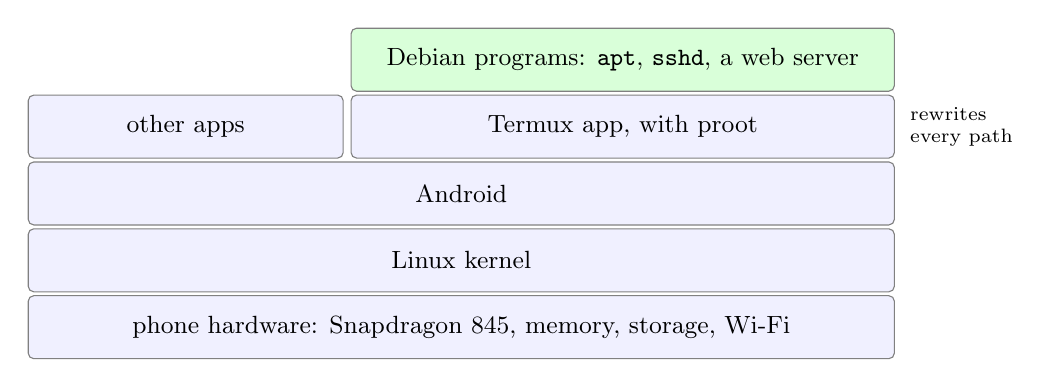
\begin{tikzpicture}[font=\small,
  layer/.style={draw=black!50, rounded corners=2pt, minimum height=0.8cm, align=center, fill=blue!6},
  deb/.style={layer, fill=green!15}]
  \node[layer, minimum width=11cm] (hw) {phone hardware: \name{Snapdragon 845}, memory, storage, Wi-Fi};
  \node[layer, minimum width=11cm, above=1pt of hw] (k) {Linux kernel};
  \node[layer, minimum width=11cm, above=1pt of k] (os) {Android};
  \node[layer, minimum width=4cm, above=1pt of os.north west, anchor=south west] (and) {other apps};
  \node[layer, minimum width=6.9cm, above=1pt of os.north east, anchor=south east] (tx) {\name{Termux} app, with \name{proot}};
  \node[deb, minimum width=6.9cm, above=1pt of tx] (d) {Debian programs: \texttt{apt}, \texttt{sshd}, a web server};
  \node[font=\scriptsize, right=2pt of tx, align=left] {rewrites\\every path};
\end{tikzpicture}
\end{center}

\here[diagram: Termux on Android] \name{Termux} is an Android app like any other, so it sits on Android, and Android decides what it may do. \name{proot} still passes each Debian program's requests to the kernel itself.

\here[three paths] Debian can run on this phone in three ways, from the lightest to the heaviest.
\begin{enumerate}[leftmargin=2em,itemsep=1pt]
\item Without root, Debian runs under \name{proot} inside \name{Termux}, as above.
\item With root, Debian runs under a real \name{chroot}, still on Android, at full speed.
\item \name{postmarketOS} replaces Android and its kernel with a Linux system for phones.
\end{enumerate}

\here[Magisk] Rooting a phone gives its apps the right to act as root. \name{Magisk} is the usual tool for it: it patches the boot image, the part of the phone's storage that starts the kernel, so that root goes only to the apps I allow, and it loads add-ons, called modules~\cite{magisk}. Rooting gives three advantages. A real \name{chroot} runs Debian programs at full speed, talking to the kernel directly. A root-only module, \name{ACC}, can hold the battery's charge below full, as the box below explains. And services can use the standard ports below 1024, which Linux reserves for root: a web server on 80 or 443, and \name{Pi-hole} on 53, the port every device asks for DNS. \name{Pi-hole} is one of the services I want, so I root the phone.\here[root: decided]

\here[erase] Rooting needs an unlocked bootloader, the program that starts the phone, and unlocking it erases the phone. The phone held only a few old apps and photos, which the next steps check before the erase. The erase also clears today's setup, which \texttt{install.sh} restores.

\here[mainline explained] The kernel under Android is OnePlus's own copy of Linux, version 4.9.227, from the kernel line of Dec 2016, to which OnePlus and Qualcomm added the drivers for this phone's chips. Those drivers live only in that copy. The mainline kernel is the official Linux, which Linus Torvalds releases at kernel.org and every Linux distribution builds on. Volunteers of \name{postmarketOS} have since written open drivers for most of the OnePlus 6 and added them to mainline, so mainline runs on the phone today. \name{postmarketOS}, a Linux distribution for phones, is built on mainline, and the OnePlus 6 (codename \name{enchilada}) runs it well~\cite{pmos}. The first two paths keep Android's kernel, with all of OnePlus's drivers; the third trades them for mainline's.

\begin{insight}{The battery}
\name{OxygenOS} 11 charges the battery to 100\% and holds it there while the phone stays plugged in, and a battery kept full for months wears out faster and can swell. Stopping the charge earlier needs root. \name{ACC} (Advanced Charging Controller), a \name{Magisk} module, stops charging at a level I choose, such as 80\%, and starts again below a lower one. \here[current cap] It can also cap the charging current, and on kernels that support it, it runs the phone straight from the charger and leaves the battery alone~\cite{acc}. Whether these hold depends on the kernel, so the next steps check them. A server wants slow charging, because it keeps the phone cool, and the generic USB-A to C cable already charges slowly; the Warp cable is for a quick top-up.
\end{insight}

\section*{Reaching the phone from the Mac}

On Tue 10 Nov the phone was plugged into \name{AlfMAC4} with a USB cable, and the Mac drove it with \name{adb}, the Android Debug Bridge, a command-line tool that runs commands on a phone over USB. \name{adb} works only after the phone allows it. Tapping \name{Build number} seven times, under \name{Settings}, \name{About phone}, \name{Version},\here[menu names] turns on \name{Developer options}, and \name{USB debugging} inside them lets \name{adb} in. The phone then asks once whether to trust this computer.

\begin{pane}
$ adb shell getprop ro.build.display.id  # which software the phone runs
\end{pane}
\begin{cmdout}
ONEPLUS A6003_22_211125
\end{cmdout}

The build ends in 211125, 25 Nov 2021, so the phone already ran the final \name{OxygenOS} 11.1.2.2, and the update step was already done. \texttt{adb shell top} showed the phone's load: 8 cores, mostly idle, and 7.4 of 7.8 GB of memory in use, which is normal on Android, because it keeps recent apps in memory. \here[memory] Android hands that memory back as soon as a program asks for it, by closing the apps it was keeping. Uninstalling the apps I never use frees what their background services hold: \texttt{adb shell pm uninstall -{}-user 0} followed by an app's package name removes even an app OnePlus preinstalled, and a factory reset brings it back.

\section*{What is inside}

\here[opening rewritten] This table names the chips around the processor and what each one does. The phone reports its own parts over \name{adb}, through \texttt{getprop}, \texttt{/proc/cpuinfo}, and \texttt{dumpsys}. Qualcomm's product brief describes the processor~\cite{qcom}. And the mainline kernel describes the whole board in a device tree, a text file that names each chip on the board, the bus it sits on, and the power supply that feeds it~\cite{dts}. \here[who wrote it] The \name{postmarketOS} volunteers wrote it from the kernel source that OnePlus publishes, as Linux's licence requires, and from testing on the phone, so it is the open counterpart of the schematics that OnePlus keeps internal.

\begin{center}\small
\here[3rd column; model, kernel moved]
\begin{tabular}{@{}lp{5.4cm}p{6.2cm}@{}}
\toprule
Part & Chip & What it does \\
\midrule
Processor (CPU) & Qualcomm \name{SDM845}, \name{Kryo} 385 cores, 10 nm & runs every program \\
Graphics (GPU) & \name{Adreno} 630, OpenGL ES 3.2 & draws the screen \\
Signal processor (DSP) & \name{Hexagon} 685 & sound, sensors, and neural networks, at low power \\
Camera processor & \name{Spectra} 280 & turns the camera sensor's raw data into photos \\
Display & Samsung AMOLED, \name{sofef00} (\name{AMS628NW01}), 1080 $\times$ 2280 & the screen \\
Touch & Synaptics \name{S3706B} & senses fingers on the screen \\
Modem & Qualcomm \name{X20} LTE & mobile data and calls, through the SIM \\
Wi-Fi and Bluetooth & Qualcomm \name{WCN3990} & the radios for both \\
NFC & NXP \name{PN553} & Near-Field Communication: contactless payments and tags, a few centimetres away \\
Power & Qualcomm \name{PM8998} & feeds every chip its voltage \\
Charging & Qualcomm \name{PMI8998} & charges the battery from the USB-C port \\
Battery gauge & Texas Instruments \name{BQ27411} & measures how much charge the battery holds \\
Speaker amplifier & Maxim \name{MAX98927} & drives the loudspeaker \\
\bottomrule
\end{tabular}
\end{center}

\here[led with the answer] Two lines of the device tree show what \name{postmarketOS}, the third path, would cost a server: mainline lacks two of OnePlus's drivers. The first switches the USB-C port to host. Under mainline the port works only as a device, the role it plays when plugged into a computer, so an SSD, an Ethernet adapter, or my own hardware on that port needs Android's kernel. The second drives Dash Charge, which charges at 4 A through the Warp adapter; mainline charges at most 1.8 A, through \name{PMI8998}. Slow charging suits a server, so only the missing host mode counts, and it keeps the first two paths, on Android's kernel, ahead.

\section*{Termux}

The phone already had \name{Termux} 0.101, installed from the Play Store in Sep 2018, and it no longer started: its shell stopped with \texttt{CANNOT LINK EXECUTABLE \ldots{} library "libandroid-support.so" not found}. \name{Termux} stopped publishing to the Play Store years ago, so that copy cannot be repaired. Its current builds are on GitHub~\cite{termux}, and the Mac installed one after the old app was removed:

\begin{pane}
$ adb install termux-app_v0.118.3+github-debug_arm64-v8a.apk  # current Termux, from GitHub
\end{pane}
\begin{cmdout}
Performing Streamed Install
Success
\end{cmdout}

Android warned that the app was built for an older version of Android. \name{Termux} declares an older version on purpose, because that is what lets it run the programs it downloads, and newer versions block that for apps declaring a recent one. Its add-ons, such as \name{Termux:Boot}, work only with a \name{Termux} from the same source, so they come from GitHub too. \here[why same source] Android lets two apps share their files only when the same key signed both, and each source signs its builds with its own key. The GitHub builds of the whole \name{Termux} project carry one shared CI debug key, and it is the key my \name{Termux} and \name{Termux:Boot} have; the same add-on from F-Droid is signed elsewhere and Android refuses it for the mismatch.

\name{Termux:API}~\cite{tapi} is the add-on that lets a program inside \name{Termux} ask Android what the sandbox keeps from an app: the battery charge, the sensors, a raw USB device~\cite{tusb}. The Mac installs it the same way as the app itself, and the phone asks for the install by hand:

\begin{pane}
$ adb install termux-api-app_v0.53.0+github.debug.apk  # Termux:API, from GitHub
\end{pane}
\begin{cmdout}
adb: failed to install ...: Failure [INSTALL_FAILED_VERIFICATION_FAILURE]
Performing Streamed Install
Success
\end{cmdout}

The first line is \name{OxygenOS} checking an app that did not arrive through the \name{Play Store}: it installs such an app only once I tap to approve it on the phone. Its answer to a battery question, \texttt{termux-battery-status}, prints the charge as JSON, and my \name{tmux} status bar below draws it as a bar of squares.

\here[htop rewritten] To watch the whole phone, \name{htop} runs through \name{adb} rather than inside \name{Termux}. \name{Termux} is an Android app, also when I reach it over SSH, and Android hides two things from apps: \begin{enumerate*}[label=(\arabic*)] \item the other apps' processes, so \name{htop} lists only \name{Termux}'s own, and \item \texttt{/proc/stat}, the kernel's file of per-core time counters from which \name{htop} works out the load, which answers \texttt{Permission denied}, so \name{htop} draws every core as offline.\end{enumerate*} Root lifts both limits. \name{adb}'s shell sees all the processes and may read the counters, and it may run programs from \texttt{/data/local/tmp}. \here[XDG] That folder belongs to Android and lies outside the XDG base directories of my lesson on where an app keeps its files, which sit in a user's home: Android sets it aside as the one place where the \name{adb} shell may write files and run them. The project's repository, \name{alfdroid}, holds this as its first tool, a script called \texttt{htop}. On its first run it copies \name{Termux}'s \name{htop} and the three libraries it needs to \texttt{/data/local/tmp/htop}, and from then on it starts \name{htop} there through \name{adb}. That folder is also \name{htop}'s home, where it saves its settings, because the shell user's own home is \texttt{/}, which it may not write.

\begin{pane}
$ ./htop  # in the alfdroid repository: all cores, all processes; q quits
\end{pane}

\section*{My settings on the phone}

The phone carries the same settings as my Macs. \texttt{pkg install git}, then a clone of my settings repository into \texttt{\textasciitilde/.settings}, and \texttt{./install.sh} in its \texttt{Termux} folder sets up the rest. The installer adds the command-line tools with \texttt{pkg}, \name{Termux}'s package manager, links my \texttt{bashrc}, Git, and Neovim settings, gives \name{Termux} the colours of my Mac's \name{Monokai} profile, and builds the terminal font, Cascadia's ExtraLight face with my pinyin patch, as on the Mac. One more setting keeps the on-screen keyboard closed until I tap the screen.

My prompt shows a user and a machine name. On the phone, \name{Termux}'s user is the app's own account, \texttt{u0\_a1}, which only root could rename, and Android keeps its device name where the prompt cannot read it. Two lines in \texttt{\$PREFIX/etc/machine-info} on the phone, \texttt{PRETTY\_HOSTNAME=AlfDROID} and \texttt{PRETTY\_USERNAME=atcold}, give the prompt its names, so it reads \texttt{atcold@AlfDROID}, as on the Macs. \here[user name over SSH] SSH logs in all the same, because \name{Termux}'s \name{sshd} serves its one user under any user name, so \texttt{ssh alfdroid} sends my Mac's name, \texttt{atcold}, and lands in \texttt{u0\_a1}.

\name{tmux} installs from the same repository: \texttt{bash \textasciitilde/.settings/Tmux/install.sh} compiles the terminal description and links the shared configuration, and under \name{Termux} it also links the phone's own status line and battery script. The bottom status row then reads its name from \texttt{machine-info}, the same file as the prompt, because Android answers \texttt{hostname} with \texttt{localhost}, and draws the charge from \name{Termux:API}; the script asks it under a two-second timeout, because the question is a broadcast to the add-on app and waits forever when no app is there to answer. Bare \texttt{tmux} opens the machine's own session, named after the display name with its \texttt{Alf} dropped, so the phone's session is \texttt{Droid} and the bar's right end reads \texttt{Droid:1.1}.

\begin{pane}
$ tmux       # into the machine's own session, Droid on this phone
\end{pane}
\begin{cmdout}
                                                   1:.settings•
AlfDROID :: ◼◼◼◼◼◼◼◼◼◼ 96% ↑                                       Droid:1.1 :: 11 Nov 2026 :: 16:01
\end{cmdout}

The phone also dials out, and its SSH client settings follow the Mac's split. The shared \texttt{ssh\_config} loads \texttt{\textasciitilde/.ssh/config.local} above its \texttt{Host} lines, because OpenSSH reads no \texttt{Host} entry from a file included inside one, and the options only \name{macOS} understands live on the Mac's own side of that split. The phone's copy of the file holds its one machine:

\begin{lstlisting}[style=out]
Host alfspark
    User atcold
\end{lstlisting}

The Spark's \name{sshd} must see a user name it accepts, and the phone's key sits in the Spark's \texttt{authorized\_keys}. With that entry, the \texttt{spark} tool of my lesson on local coding runs unchanged on the phone: \texttt{spark serve tunnel} opens the phone's own pipe to a serving Spark, and the plug account's password, which on the Mac lives in the Keychain, sits here in \texttt{\textasciitilde/.config/spark/credentials.toml} under mode 600.

\section*{Reaching it from anywhere}

The \name{Tailscale} app joined the phone to the tailnet as \texttt{oneplus-6}, the name it took at its first login, and the admin console renamed it \texttt{alfdroid}. \name{Termux}'s SSH server, \name{sshd}, listens on port 8022, because without root it may use only ports above 1024. Two lines in my Mac's SSH settings, \texttt{Host alfdroid} and \texttt{Port 8022}, make \texttt{ssh alfdroid} work like \texttt{ssh alfspark}.

\here[numbered list] After a reboot three things have to come back by themselves.
\begin{enumerate}[leftmargin=2em,itemsep=1pt]
\item \name{Termux:Boot}~\cite{boot} runs the scripts in \texttt{\textasciitilde/.termux/boot} when the phone starts, and mine runs \texttt{termux-wake-lock}, then \texttt{sshd}. Android lets it do that only after the app has been opened once. \here[wake lock] The wake lock keeps the processor awake while the screen stays off, so the phone never sleeps while it serves. Any app may hold one without root, the way a music player keeps playing with the screen off, and \name{Termux} shows a notification while it does.
\item \name{Tailscale} has to be the always-on VPN, which Android starts at boot, and both apps have to be exempt from battery optimisation. Android, and OnePlus's own battery manager on top of it, holds back the apps that are not exempt while the phone sits idle after a boot. Before the exemption, \name{Tailscale} stayed offline after a reboot until something woke the phone, and every \name{adb} command did.
\item The screen lock has to be \name{None}.\here[None] With a PIN, Android keeps every app's data encrypted after a reboot until someone types the PIN, and both \name{Termux} and \name{Tailscale} keep their data there, so neither can start. With the lock set to \name{None}, the data unlocks itself at boot. That also lets anyone holding the phone into it, so LastPass and the other personal accounts left the phone first. With the lock still on, a reboot followed by an unlock and nothing else brought \name{Tailscale} up, and \texttt{ssh alfdroid} answered two minutes after the restart.
\end{enumerate}

\name{adb} sets the VPN and the exemptions:

\begin{pane}
$ adb shell settings put secure always_on_vpn_app com.tailscale.ipn  # Tailscale starts at every boot
$ adb shell dumpsys deviceidle whitelist +com.tailscale.ipn  # exempt Tailscale from battery optimisation
$ adb shell dumpsys deviceidle whitelist +com.termux  # and Termux
$ adb shell settings put global auto_time 1  # set the clock from the network
\end{pane}

\here[install.sh with root] With root, \texttt{install.sh} can run the same four settings on the phone itself through \texttt{su}, so a fresh install needs no Mac.

The last line came from a commit that \texttt{git lg} on the phone listed as made ‘in the future’. The phone's automatic time was off, and its clock ran half a minute behind the Mac's, so a commit made on the Mac seconds earlier was still ahead of the phone's clock. With network time on, both clocks read the same.

\section*{The USB-C port}

The cable goes into the phone at a slant, with one side deeper than the other, and holds loosely, while the same cable clicks into the Mac. The port looks clean, so its metal shell or the contact tongue inside is probably bent. \name{adb} still sees the phone through it. \here[power cable; port board] A server needs a port that holds its power cable firmly. The port sits on a small board at the bottom of the phone, and iFixit replaces that board in about 40 minutes, opening the phone from the back~\cite{ifixit}.

\section*{Next steps}

\here[steps updated]
\begin{enumerate}[leftmargin=2em,itemsep=1pt]
\item Look at the USB-C port under the microscope, and replace its board if the tongue or the shell is bent.
\item Ask the carrier for a second, physical nano-SIM on my plan, so the phone stays online over mobile data in a power cut.
\item Find out whether the JBL speaker can be switched on over Bluetooth.
\item Note the apps still on the phone and check that its photos are backed up.
\item Unlock the bootloader, which erases the phone, install \name{Magisk}, and add the \name{ACC} module with a charge limit of 80\% and a low charging current. Leave the phone plugged in for a day and check that the charge stays there.
\item Restore the setup: \texttt{./install.sh}, with the four settings above moved into it through \texttt{su}, and \name{Termux:Boot} opened once.
\item Run \texttt{proot-distro install debian}, then \texttt{proot-distro login debian}, which opens a Debian shell with \texttt{apt}.
\end{enumerate}

\section*{What it can run}

The first service is a web server on the tailnet, for a landing page or an API. \name{Home Assistant}, a home-automation hub, can switch the Wi-Fi plugs over the LAN. With an SSD on the USB-C port, \name{Nextcloud} or a plain file share turns the phone into a NAS (Network-Attached Storage),\here[NAS; sync] a file server for the house. Such a server could replace Dropbox for my files. A sync conflict comes from two machines writing their own copies of the same file before either sees the other's change, and settings files are written often. A sync service of my own, such as \name{Syncthing} or \name{Nextcloud}, copies files the same way and keeps both versions of a conflict, as Dropbox does. A network share keeps a single copy, on the phone, which both Macs open over the tailnet, so every write lands in that one file; it works only while the Mac reaches the phone. \name{Pi-hole} or \name{AdGuard Home} answers the network's DNS lookups and blocks the ones that go to ad servers, for every device at once. \name{AlfBOT} can run here too, so it answers even when both Macs sleep. \here[music] And the phone can play music on the Bluetooth speaker.

\begin{thebibliography}{iFixit}
  \bibitem[RPi]{rpi} Raspberry Pi, \textit{A new 3GB Raspberry Pi 4 for \$83.75, and more memory-driven price increases}, 1 Apr 2026. \url{https://www.raspberrypi.com/news/a-new-3gb-raspberry-pi-4-for-83-75-and-more-memory-driven-price-increases/}
  \bibitem[ACC]{acc} VR-25, \textit{Advanced Charging Controller}. \url{https://github.com/VR-25/acc}
  \bibitem[GSM]{gsm} GSMArena, \textit{OnePlus 6}, full specifications. \url{https://www.gsmarena.com/oneplus_6-9109.php}
  \bibitem[9to5]{nine} 9to5Google, \textit{OnePlus officially ends software support for OnePlus 6/6T series}, 17 Jan 2022. \url{https://9to5google.com/2022/01/17/oneplus-officially-ends-software-support-for-oneplus-6-6t-series/}
  \bibitem[Tx]{termux} Termux, \textit{Installation}. \url{https://github.com/termux/termux-app#installation}
  \bibitem[TxUSB]{tusb} Termux wiki, \textit{Termux-usb}. \url{https://wiki.termux.com/wiki/Termux-usb}
  \bibitem[TxAPI]{tapi} Termux, \textit{Termux:API}. \url{https://github.com/termux/termux-api}
  \bibitem[Qcom]{qcom} Qualcomm, \textit{Snapdragon 845 Mobile Platform}, product brief, May 2018. \url{https://www.qualcomm.com/content/dam/qcomm-martech/dm-assets/documents/qcomm_4743_845productbrief_may2018.pdf}
  \bibitem[DTS]{dts} Linux kernel, \textit{sdm845-oneplus-enchilada.dts} and \textit{sdm845-oneplus-common.dtsi}, the OnePlus 6 device tree. \url{https://github.com/torvalds/linux/blob/master/arch/arm64/boot/dts/qcom/sdm845-oneplus-common.dtsi}
  \bibitem[Boot]{boot} Termux, \textit{Termux:Boot}. \url{https://github.com/termux/termux-boot}
  \bibitem[iFixit]{ifixit} iFixit, \textit{OnePlus 6 Charging Port Replacement}. \url{https://www.ifixit.com/Guide/OnePlus+6+Charging+Port+Replacement/145810}
  \bibitem[PD]{proot} Termux, \textit{proot-distro}. \url{https://github.com/termux/proot-distro}
  \bibitem[pmOS]{pmos} postmarketOS wiki, \textit{OnePlus 6 (oneplus-enchilada)}. \url{https://wiki.postmarketos.org/wiki/OnePlus_6_(oneplus-enchilada)}
  \bibitem[Magisk]{magisk} topjohnwu, \textit{Magisk}. \url{https://github.com/topjohnwu/Magisk}
\end{thebibliography}

\end{document}
